% ============================================================
\section{The StatLM Method}
\label{sec:method}
% ============================================================
StatLM uses the three-layer encoder-decoder architecture in Fig.~\ref{fig:arch}.
Two encoder layers summarize each document and extract keyphrases; the LLM decoder
then constructs the label space and assigns labels. New batches are matched to the
existing label space, while unmatched documents form new clusters. Although the
linguistic tools and embeddings are pretrained, no domain-specific labeled data are
used for label discovery or classification.

\begin{figure*}[!t]
\centering
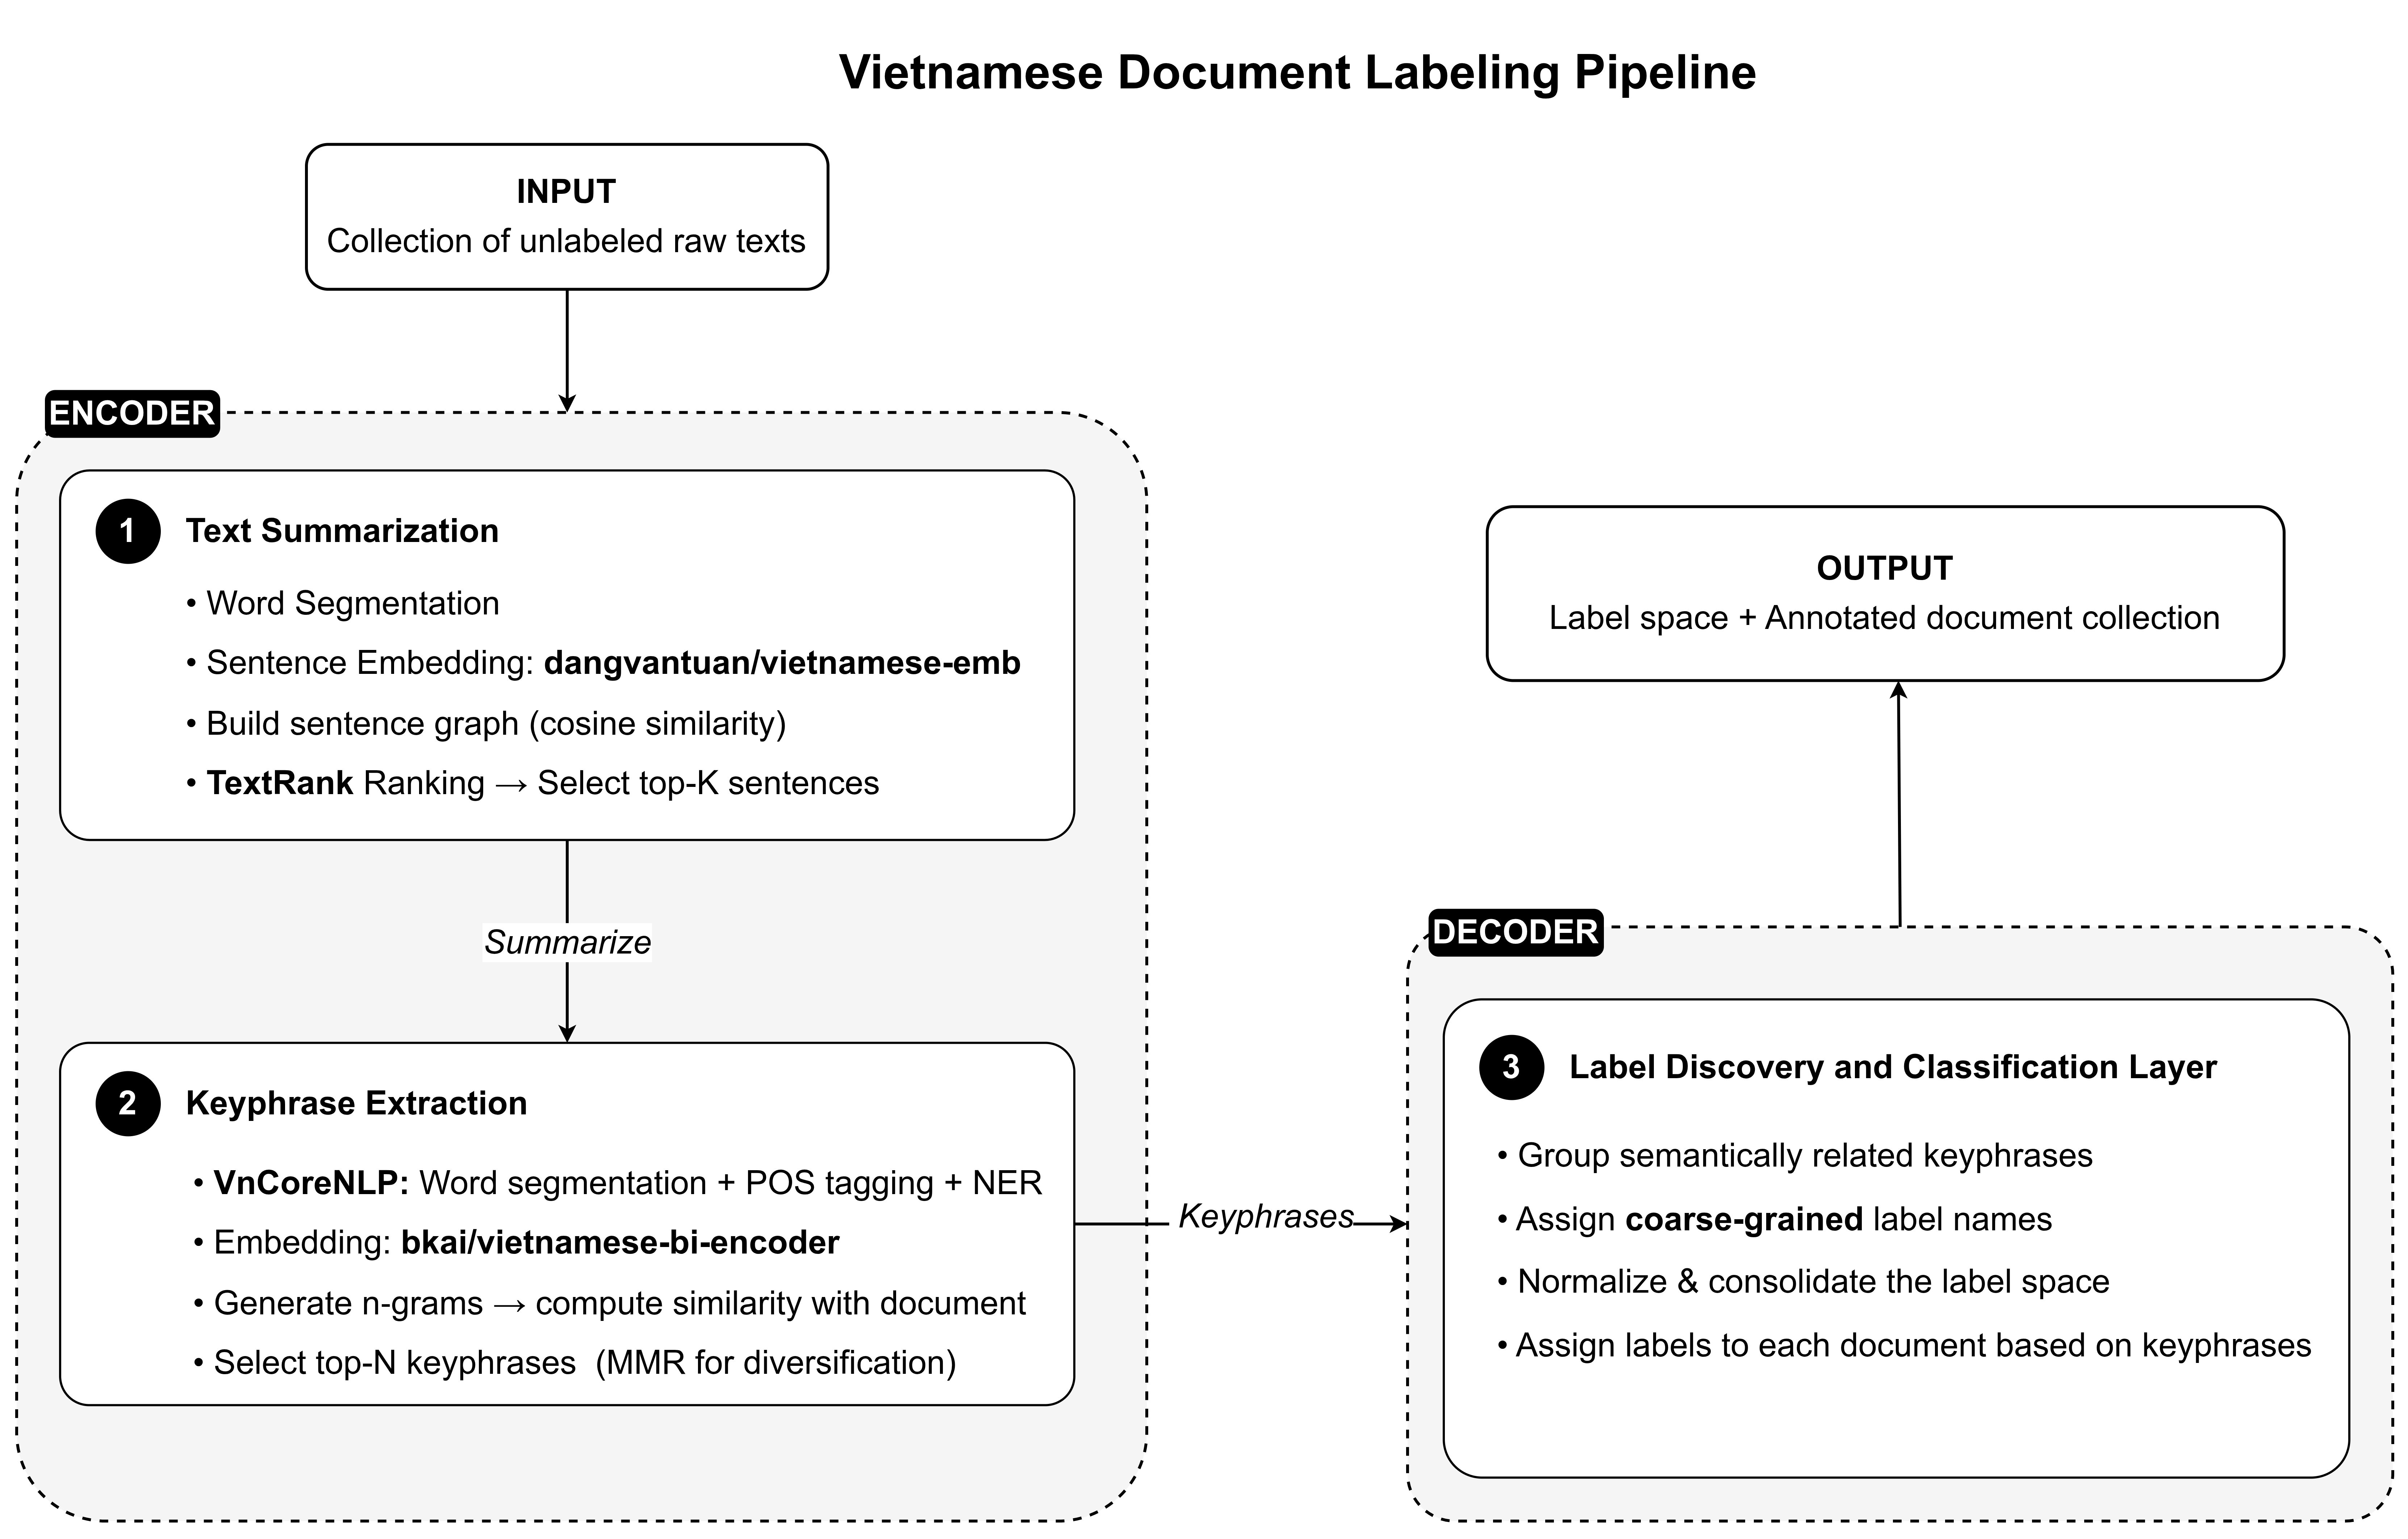
\includegraphics[width=0.93\textwidth]{figures/overview.png}
\caption{StatLM architecture: two statistical encoder layers condense each
document before the LLM decoder constructs, normalizes, and assigns labels.}
\label{fig:arch}
\end{figure*}
% \begin{figure*}[!t]
% \centering
% 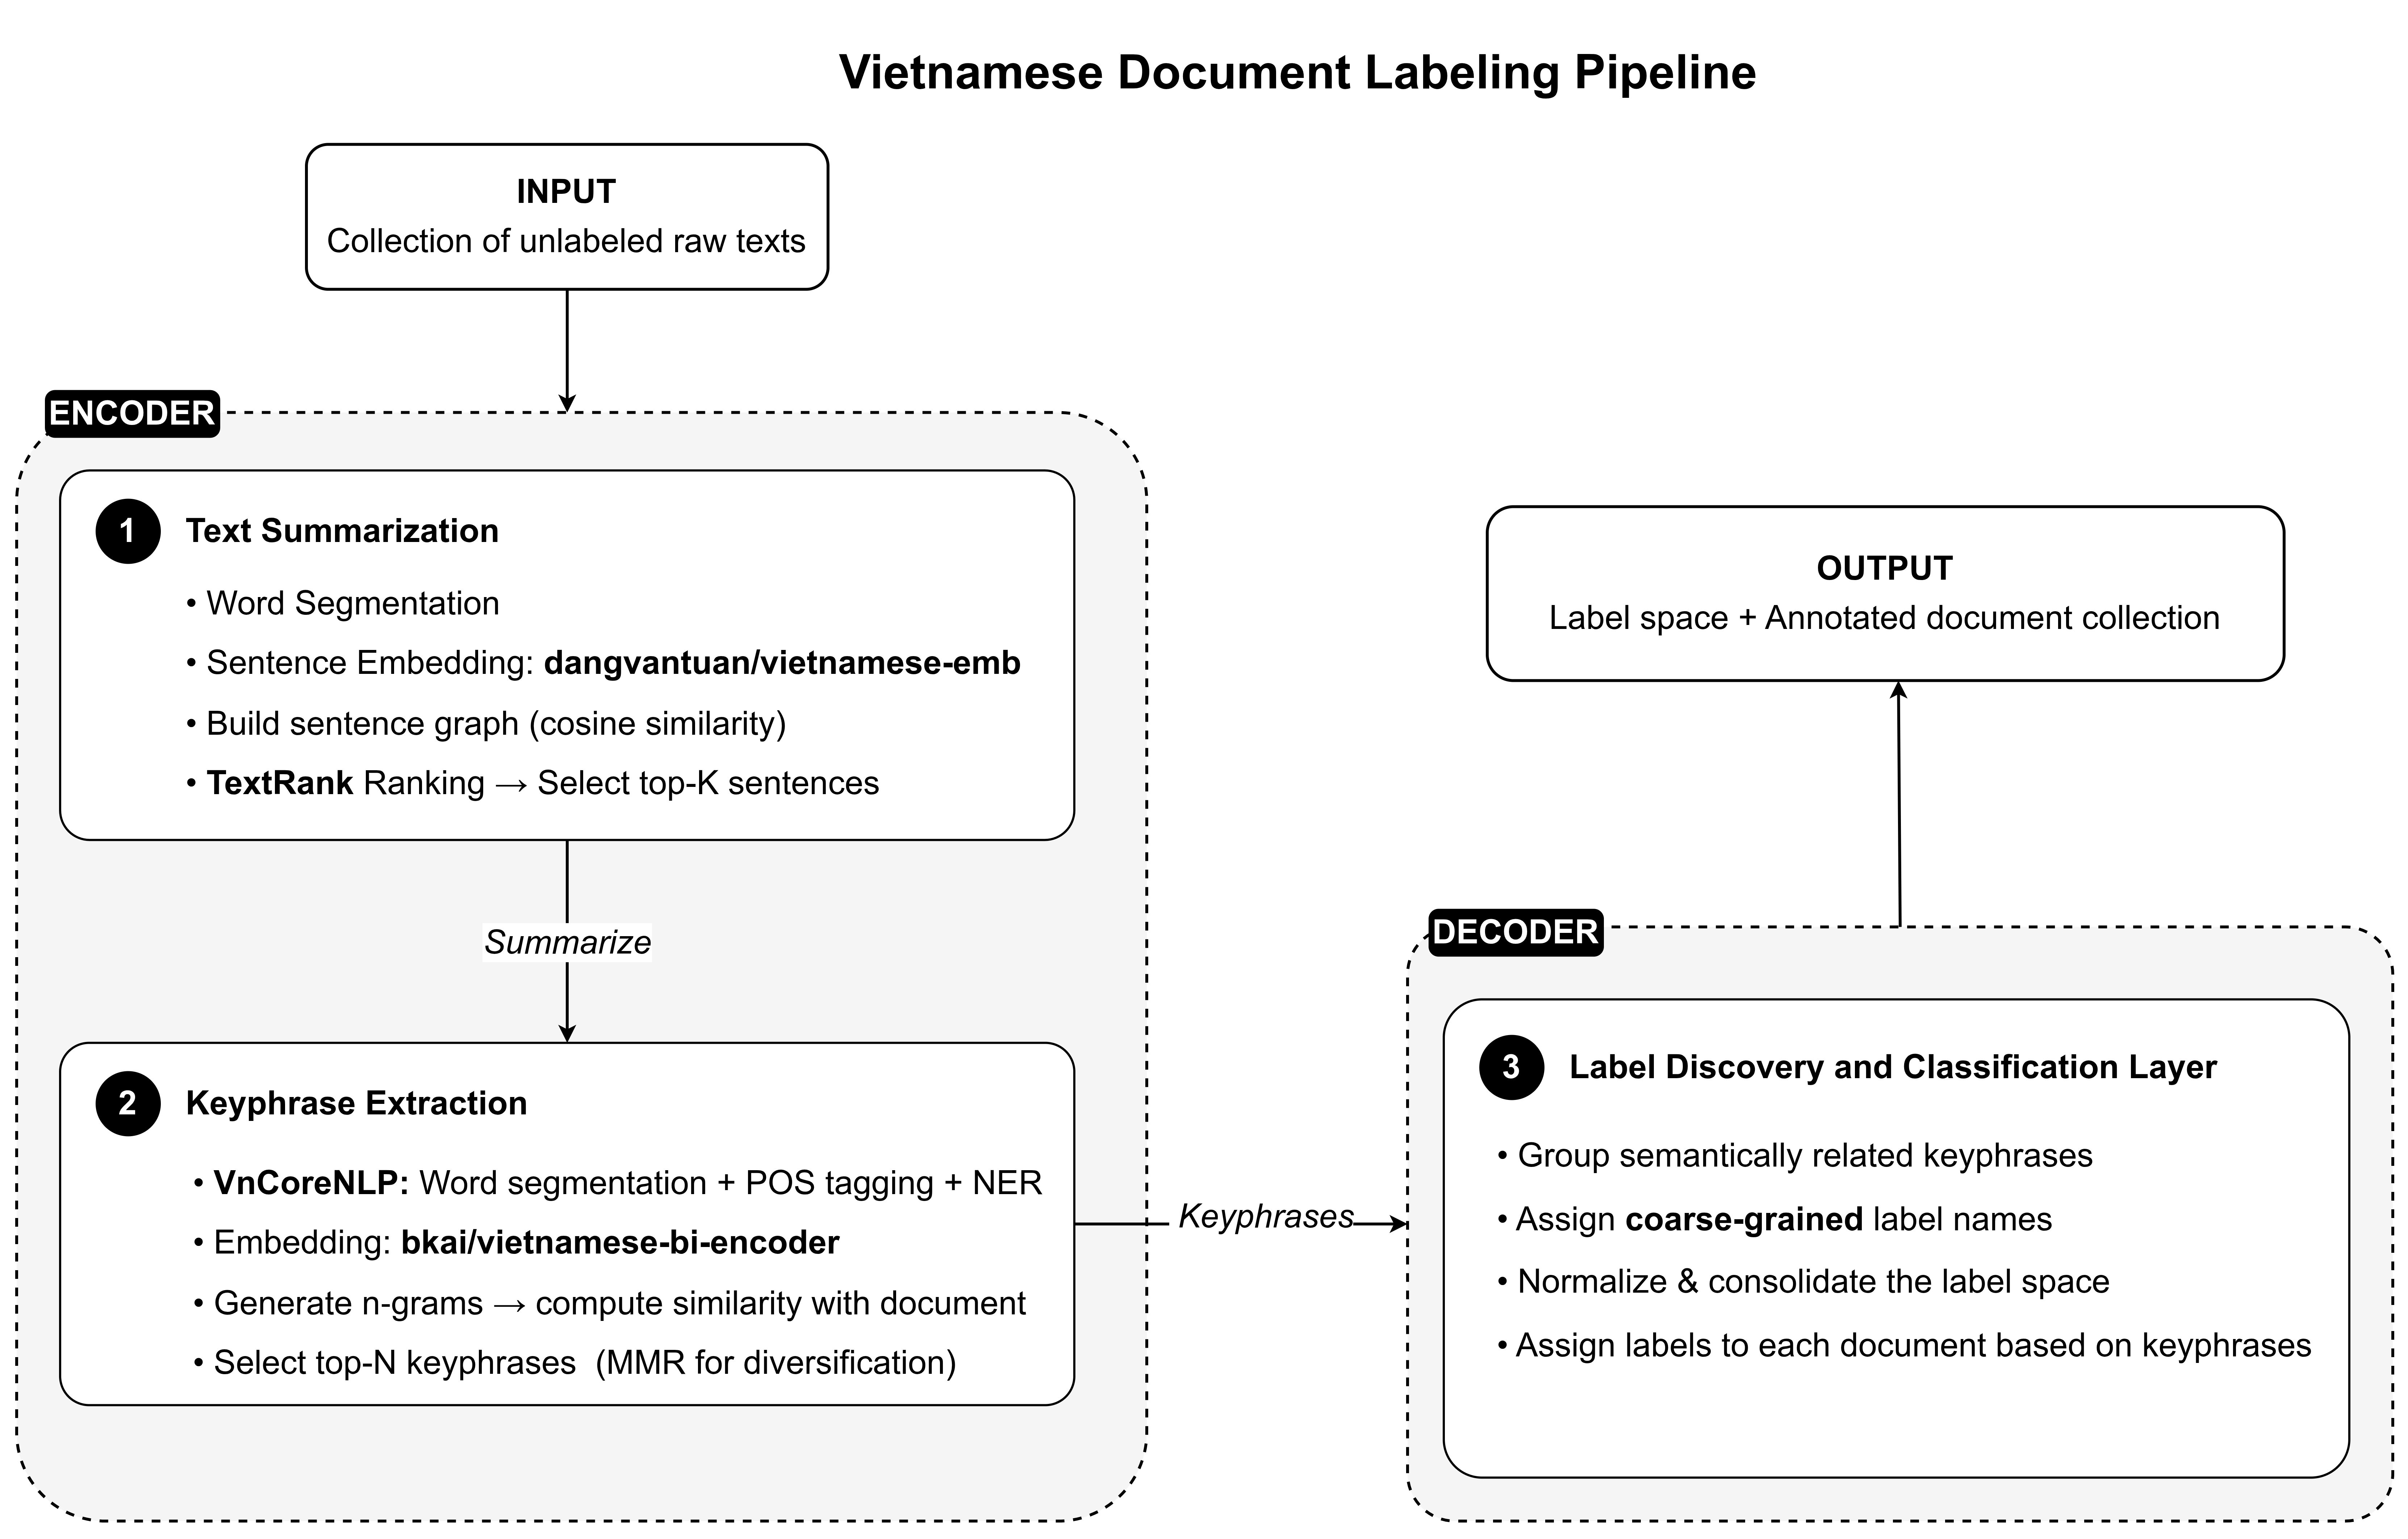
\includegraphics[width=0.95\textwidth]{figures/overview.png}
% \caption{Overall architecture of StatLM: the statistical encoder has two layers
% (summarization with TextRank + \emph{dangvantuan/vietnamese-embedding}; keyphrase
% extraction with KeyBERT + \emph{bkai/vietnamese-bi-encoder} and VnCoreNLP) that
% reduce noise and condense the information; the LLM decoder (Gemini) is invoked
% only once at the end to discover, name, and normalize the label space and to
% assign labels to each document.}
% \label{fig:arch}
% \end{figure*}

\subsection{Layer 1: Text Summarization}
For document $D=\{s_1,\ldots,s_n\}$, Layer~1 produces summary
$S=\{s'_1,\ldots,s'_k\}$, where $k<n$. StatLM applies TextRank with semantic edge
weights rather than word overlap or other lexical similarities. Because the layer
compares sentences of similar length, it uses the symmetric-STS model
\emph{dangvantuan/vietnamese-embedding}~\cite{dangvantuan2021vietnamese} with pyvi
preprocessing.

The document is split into sentences and segmented with pyvi. Each sentence is
encoded as $\mathbf{e}_i=\mathrm{meanpool}(\mathrm{PhoBERT}(s_i))\in
\mathbb{R}^{768}$, and a complete graph is built with
$W_{ij}=\cos(\mathbf{e}_i,\mathbf{e}_j)$. TextRank computes
\begin{equation}
\begin{aligned}
\mathrm{WS}(v_i)^{(t+1)} &=(1-d)+d\!\!\sum_{v_j\in\mathrm{In}(v_i)}
\frac{w_{ji}}{\sum_{v_k\in\mathrm{Out}(v_j)}w_{jk}}\\
&\quad\times\mathrm{WS}(v_j)^{(t)},
\end{aligned}
\label{eq:textrank}
\end{equation}
with $d=0.85$ and convergence threshold $\varepsilon=10^{-5}$. For $n>5$, the
$k=\max(5,\lceil0.4n\rceil)$ highest-ranked sentences are retained and restored to
their original order.

\begin{figure}[!t]
\centering
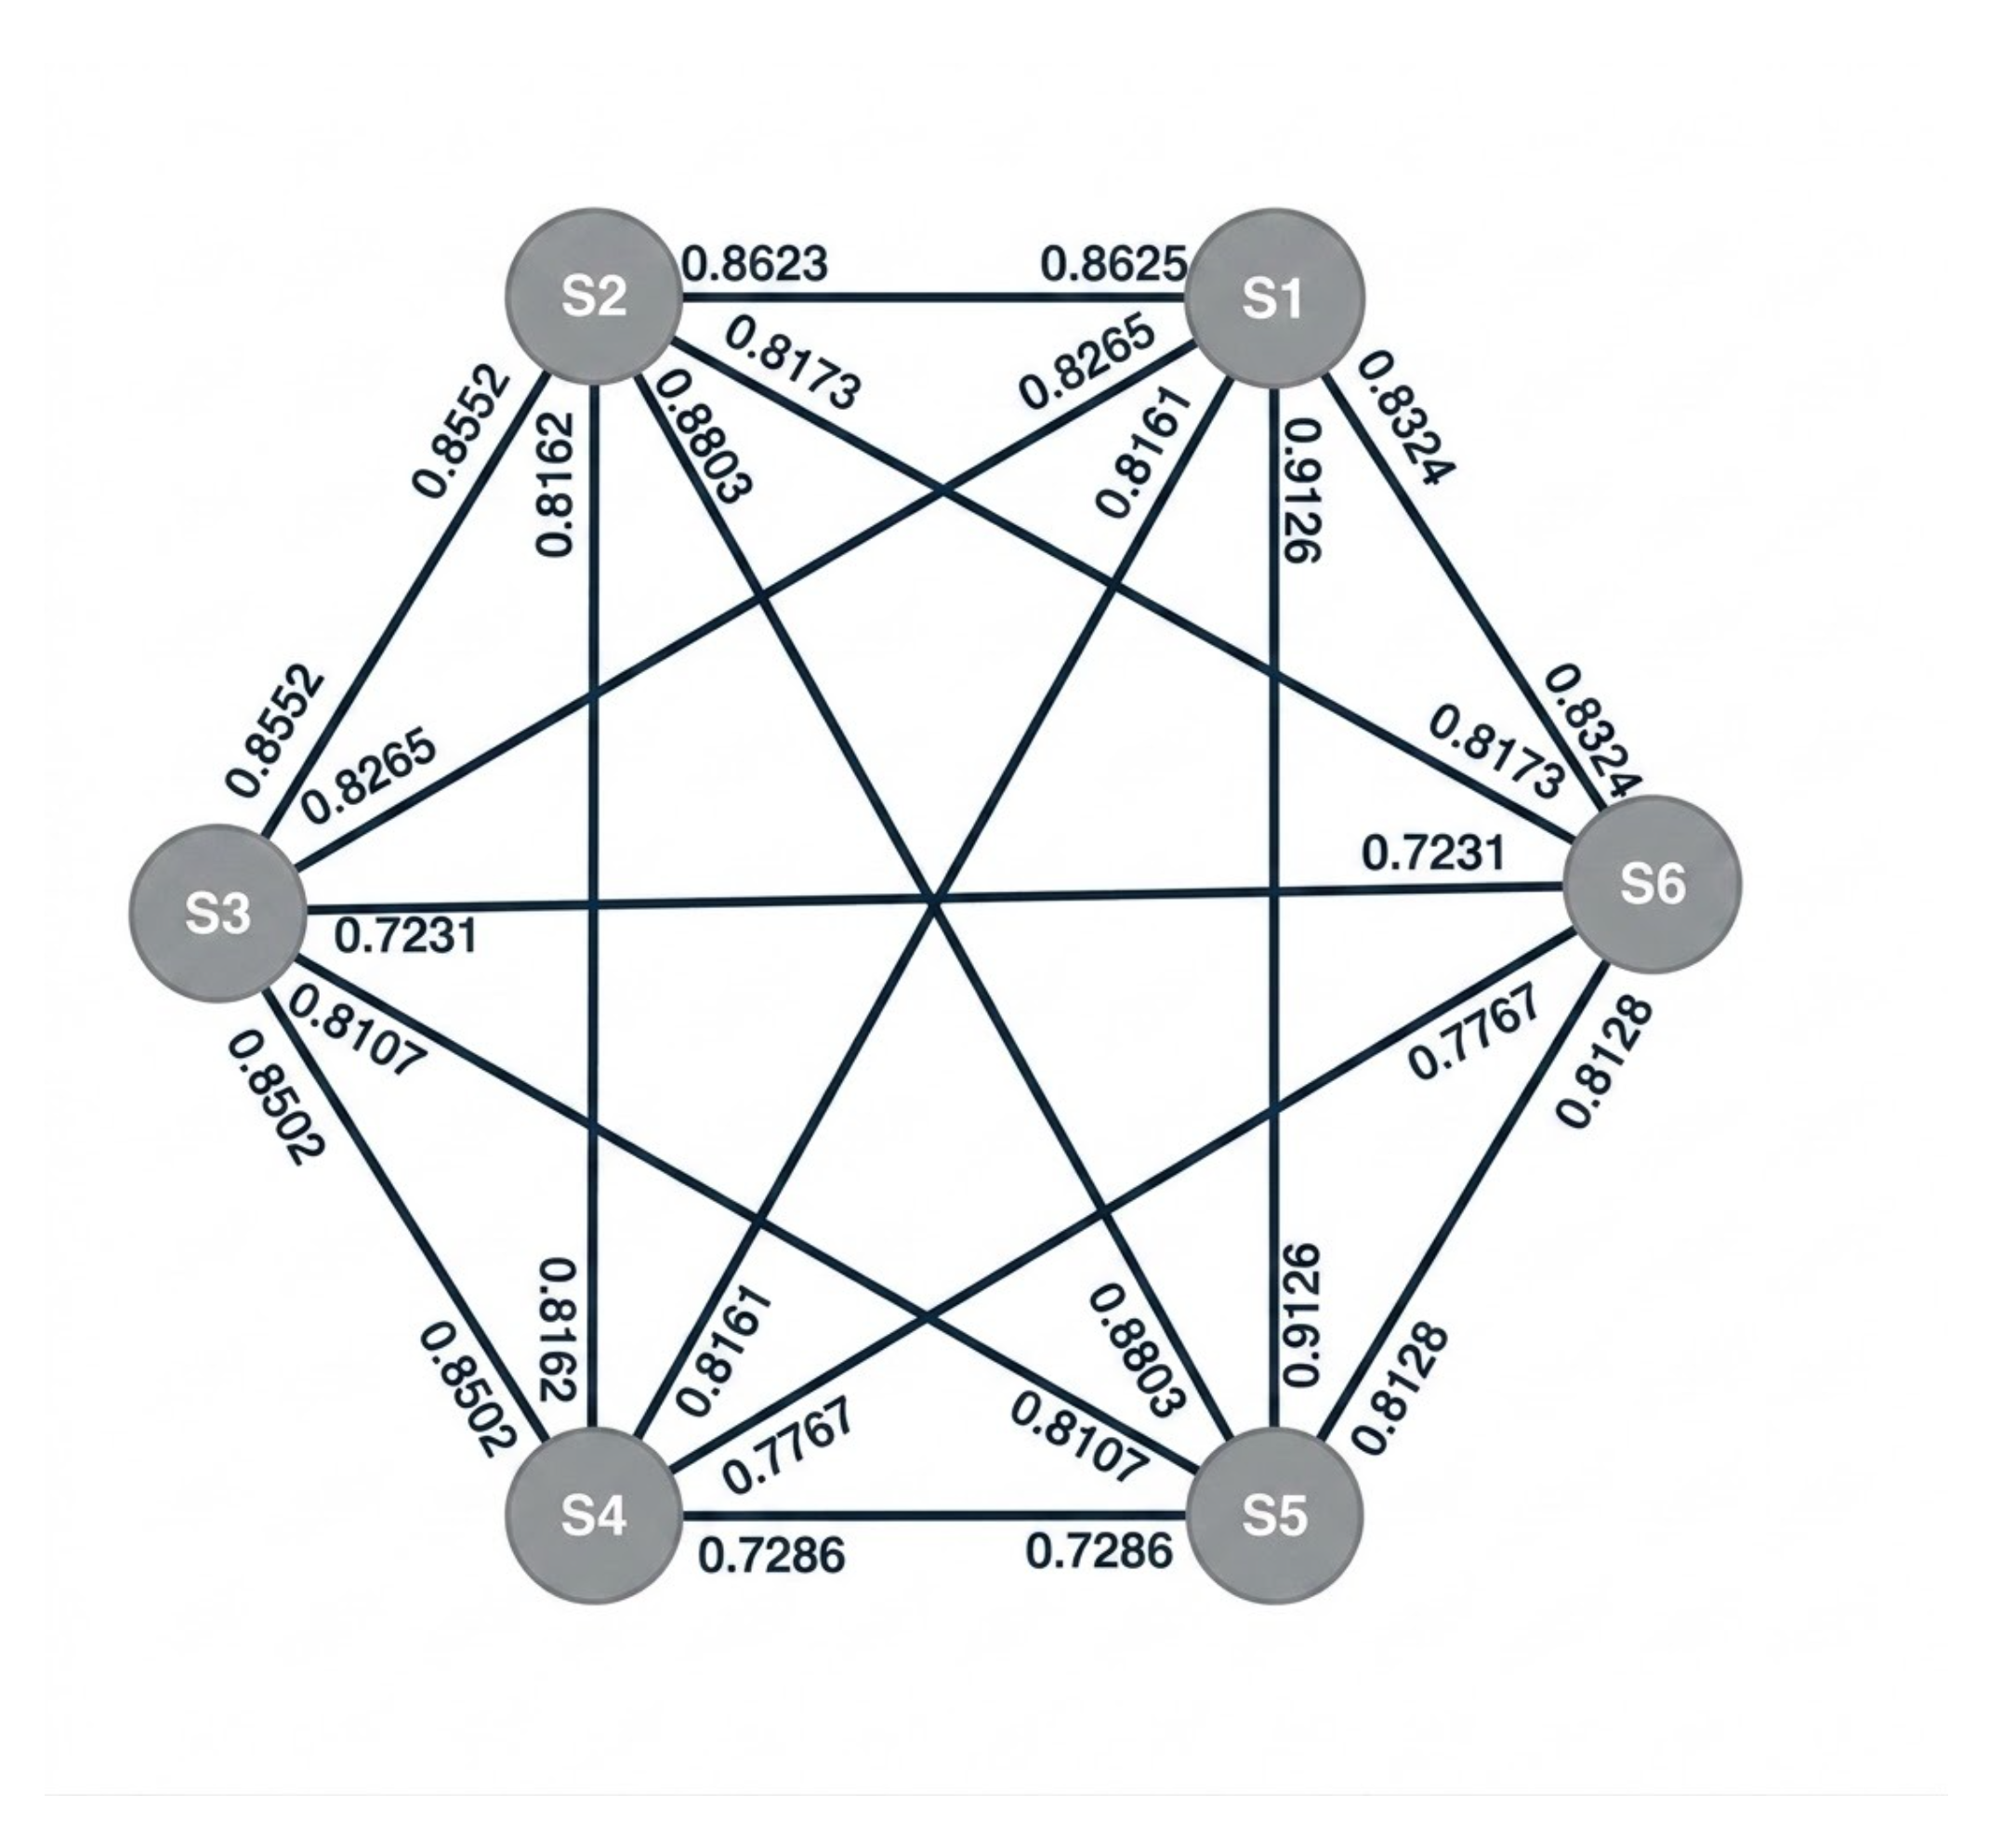
\includegraphics[width=0.95\columnwidth]{figures/stage1.png}
\caption{Layer~1 ranks a semantic sentence graph with TextRank and retains the
top-$k$ sentences.}
\label{fig:textrank}
\end{figure}

The canonical PageRank/TextRank value is fixed as $d=0.85$ because the $(1-d)$ teleportation term only keeps the walk ergodic and the ranking is documented to be insensitive to $d$ over $[0.8,0.9]$. Dataset-specific fusion schemes
~\cite{vora2024extractive} are omitted so that the retention ratio $r$ remains the
principal Layer~1 parameter. 

A sentence's score accumulates its weighted semantic similarity to the rest of the document, so the roughly 60\% discarded are low-centrality nodes such as redundant restatements, transitions, boilerplate, or peripheral asides. A recurring main subject is effectively preserved, whereas a secondary subject confined to a few low-centrality sentences may fall below the cut and cannot be recovered downstream. A sweep over $r\in[0.2,0.6]$ (Table~\ref{tab:retention}) shows closeness to the title-and-SAPO lead decreasing while topical coverage rises, so the proportional budget $k=\max(5,\lceil0.4n\rceil)$ is adopted, consistent with embedding-based TextRank outperforming Lead-$K$ on ROUGE (Table~\ref{tab:rouge}).


\subsection{Layer 2: Keyphrase Extraction}

Layer~2 extracts $m=10$ one-to-three-word keyphrases from $S$ using KeyBERT
~\cite{grootendorst2020keybert} and the asymmetric retrieval model
\emph{bkai-foundation-models/vietnamese-bi-encoder}
~\cite{nguyen2025improving}. VnCoreNLP~\cite{vu2018vncorenlp} supplies POS tags and
NER spans. Candidate n-grams are generated within sentence boundaries, filtered by
stopwords and POS tags, and supplemented with complete named-entity spans.

The procedure is: (1) preprocess with VnCoreNLP, remove stopwords, and filter by POS; (2) encode the summary into $\mathbf{E}_{doc}$; (3) generate one-to-three-word candidate n-grams within sentence fragments, adding NER entities; (4) compute
\begin{equation}
\cos(\mathbf{E}_{doc},\mathbf{E}_{ngram})=
\frac{\mathbf{E}_{doc}\cdot\mathbf{E}_{ngram}}
{\lVert\mathbf{E}_{doc}\rVert\,\lVert\mathbf{E}_{ngram}\rVert};
\label{eq:cosine}
\end{equation}
and (5) select keyphrases with MMR~\cite{carbonell1998use}:
\begin{equation}
\mathrm{MMR}=\arg\max_{c\notin S}\Big[\lambda\,\mathrm{sim}(c,doc)
-(1-\lambda)\max_{s\in S}\mathrm{sim}(c,s)\Big],
\label{eq:mmr}
\end{equation}
with $\lambda=0.5$ and redundancy cap $\theta=0.7$. The neutral midpoint is used because the top-5 keyphrases must jointly span a document's facets: emphasizing relevance yields near-duplicates, whereas emphasizing diversity admits loosely related phrases that become decoder noise. The hard cap removes a candidate whose cosine to an already selected phrase exceeds $\theta$, preserving adjacent facets while suppressing paraphrases and head-sharing substrings. With POS- and NER-filtered candidates, selection is stable around $(\lambda,\theta)=(0.5,0.7)$.

\begin{figure*}[!t]
\centering
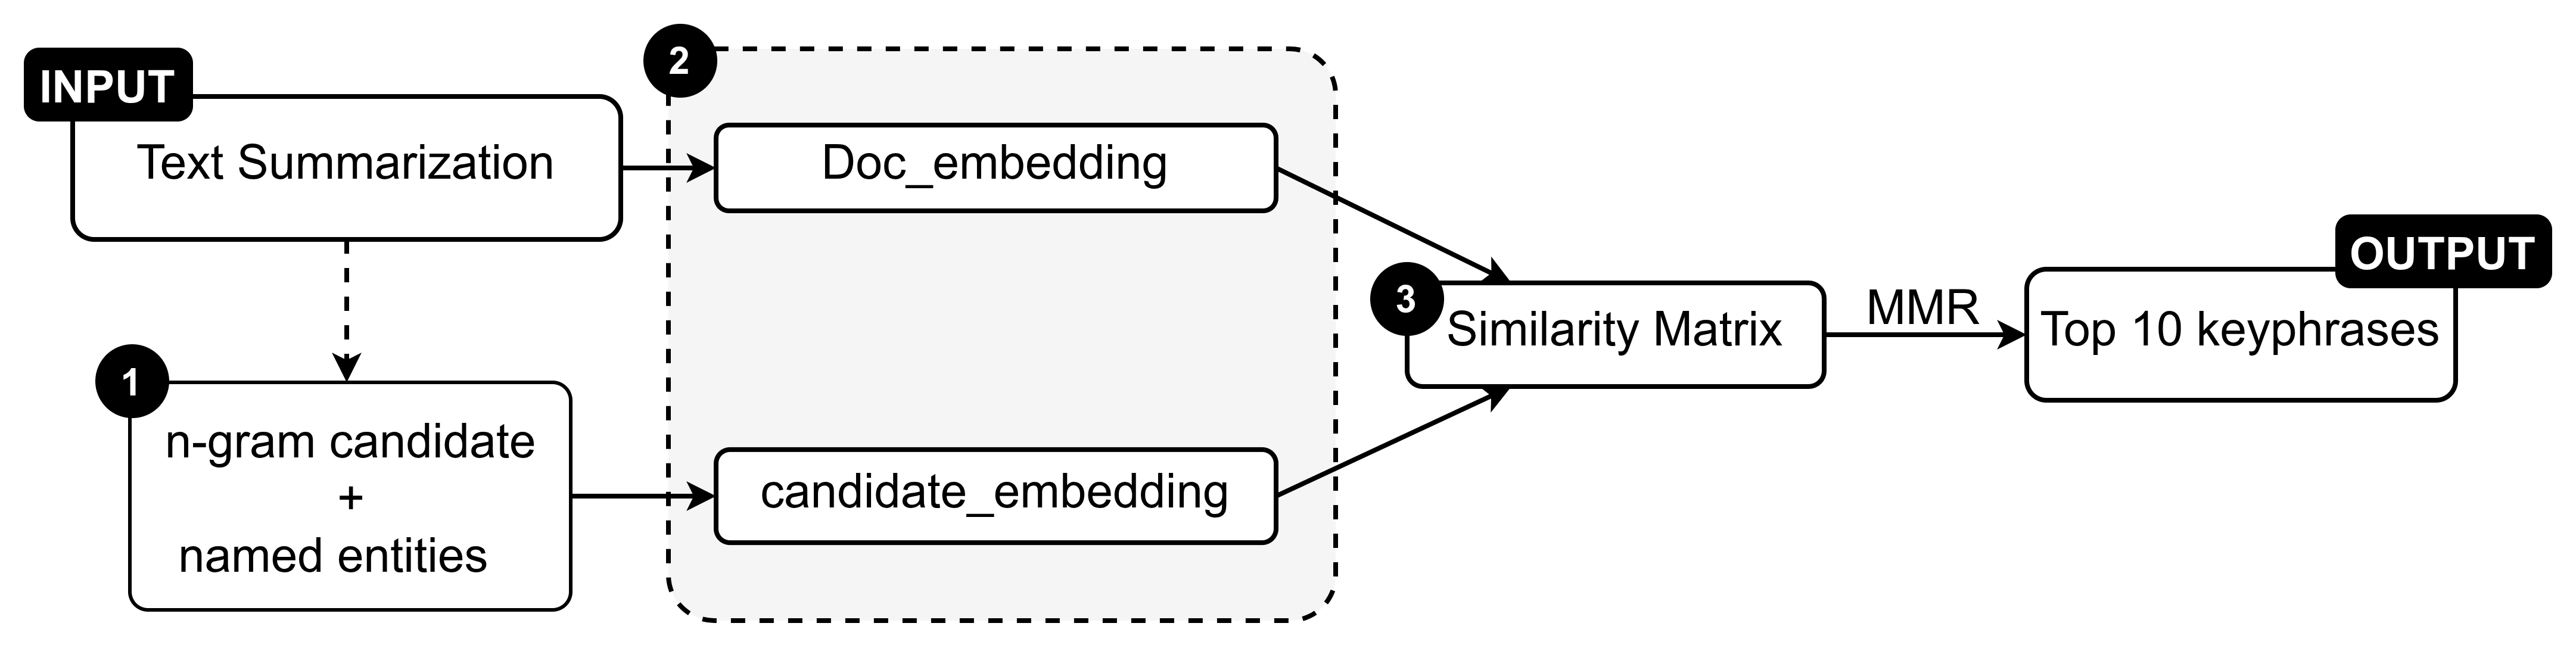
\includegraphics[width=0.8\textwidth]{figures/stage2.png}
\caption{Layer~2 encodes the summary and candidate n-grams independently, then
uses cosine ranking and MMR to select diverse keyphrases.}
\label{fig:keybert}
\end{figure*}

\begin{table}[!t]
\renewcommand{\arraystretch}{1.25}
\caption{Embedding Models Used by the Two Encoder Layers}
\label{tab:emb}
\centering
\scriptsize
\begin{tabularx}{\columnwidth}{@{}lXX@{}}
\toprule
\textbf{Criterion} & \textbf{Layer 1 (TextRank)} & \textbf{Layer 2 (KeyBERT)} \\
\midrule
Problem type & Symmetric STS & Asymmetric retrieval \\
Relation     & Sentence to sentence & Keyphrase to document \\
Model        & dangvantuan embedding & bkai bi-encoder \\
Tokenizer    & pyvi & VnCoreNLP \\
Score        & Pearson 84.21 & First on VCS retrieval \\
\bottomrule
\end{tabularx}
\end{table}

\subsection{Layer 3: Classification and Labeling with the LLM}
Given the keyphrase set $\mathcal{P}=\{p_1,\dots,p_N\}$ of $N$ documents, this layer discovers the label space $\mathcal{L}=\{l_1,\dots,l_M\}$ and assigns labels. StatLM places Gemini 2.5 Flash at the decoder after filtering and condensation, so far fewer tokens reach the API and source entities or formatting are less likely to induce noisy labels. It supports new and incremental data in three steps: (1) send only the top-5 keyphrases per document for normalization; (2) assign documents to existing clusters under a strict policy, allowing label-rename suggestions and routing non-matches to an ``unassigned'' list; and (3) cluster and name the unassigned documents. A System Message requests coarse-grained labels, avoids entity-like labels (e.g., ``Giáo dục''/``Education'' rather than ``Tuyển sinh đại học 2024''/``University Admissions 2024''), minimizes label count, and merges similar topics.

